% ARPEGOS:  Automatized Roleplaying-game Profile Extensible Generator Ontology based System %
% Author : Alejandro Muñoz Del Álamo %
% Copyright 2019 %

% Section 7.1: Entorno de Pruebas %
\section{Organización del código fuente}
Como se ha comentado en capítulos anteriores, el proyecto se ha desarrollado en \textit{Visual Studio}, y se ha aplicado el 
patrón de arquitectura \textit{MVVM}. \medskip

Al haber utilizado \textit{Visual Studio}, la aplicación se ha desarrollado en una \textbf{\textit{solución}}, que es un contenedor que contiene 
uno o más proyectos relacionados, junto a información de compilación, la configuración de \textit{Visual Studio} y archivos no asociados 
a un proyecto determinado. Por otro lado, un \textbf{\textit{proyecto}} es el conjunto de ficheros que se compilan en un archivo ejecutable, 
biblioteca o sitio web. \medskip

En lo referente a la solución diseñada, llamada {\textit{ARPEGOS}, disponemos de tres proyectos generales: \textit{ARPEGOS}, 
\textit{ARPEGOS\_Android} y \textit{ARPEGOS\_Unit\_Test}, tal y como se muestra en la figura\ref*{SolutionProjects}. Aparece además, 
otro proyecto llamado \textit{ARPEGOS\_iOS}, que indica que se puede desarrollar la aplicación también para \textit{iOS}, ya 
que \textit{Xamarin} permite desarrollar aplicaciones multiplataforma.


\begin{figure}[H]
    \centering
    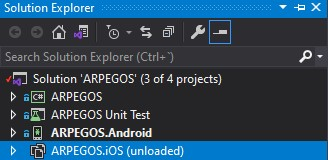
\includegraphics[scale=1.5]{Images/Solution_Projects.jpg}
    \caption{Proyectos de la solución \textit{ARPEGOS}}
    \label{SolutionProjects}    
\end{figure}

\subsection{El proyecto \textit{ARPEGOS}}
El proyecto \textit{ARPEGOS} constituye la base de la aplicación, puesto que contiene toda la lógica de negocio de la aplicación, 
independiente del dispositivo en el que se vaya a ejecutar. En la figura\ref*{SolutionARPEGOS} se muestra la estructura de este proyecto.

\begin{figure}[H]
    \centering
    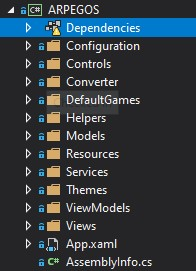
\includegraphics[scale=1.5]{Images/Solution_ARPEGOS_Project.jpg}
    \caption{Proyecto \textit{ARPEGOS}}
    \label{SolutionARPEGOS}    
\end{figure}
\newpage

\subsubsection{Configuration}
En la carpeta \textit{Configuration}, se encuentra la clase \textit{Context}, que modela 
el contexto de ejecución de la aplicación (Figura \ref*{Configuration}).

\begin{figure}[H]
    \centering
    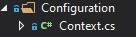
\includegraphics[scale=1.5]{Images/ARPEGOS_Configuration.jpg}
    \caption{Directorio \textit{Configuration} del proyecto \textit{ARPEGOS}}
    \label{Configuration}    
\end{figure}

\subsubsection{Controls}
El directorio \textit{Controls} contiene los distintos elementos gráficos diseñados para la aplicación (Figura \ref*{Controls}).

\begin{figure}[H]
    \centering
    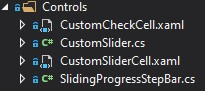
\includegraphics[scale=1.5]{Images/ARPEGOS_Controls.jpg}
    \caption{Directorio \textit{Controls} del proyecto \textit{ARPEGOS}}
    \label{Controls}    
\end{figure}

\subsubsection{Converters}
Los \textit{Converters} realizan conversiones de tipos de datos (Figura \ref*{Converters}).

\begin{figure}[H]
    \centering
    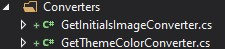
\includegraphics[scale=1.5]{Images/ARPEGOS_Converters.jpg}
    \caption{Directorio \textit{Converters} del proyecto \textit{ARPEGOS}}
    \label{Converters}    
\end{figure}
\newpage
\subsubsection{DefaultGames}
Este directorio contiene la información de los juegos por defecto (Figura \ref*{DefaultGames}).

\begin{figure}[H]
    \centering
    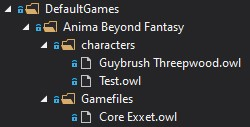
\includegraphics[scale=1.5]{Images/ARPEGOS_DefaultGames.jpg}
    \caption{Directorio \textit{DefaultGames} del proyecto \textit{ARPEGOS}}
    \label{DefaultGames}    
\end{figure}

\subsubsection{Helpers}
Esta carpeta contiene elementos que proveen funcionalidades que no 
forman parte de los objetivos de la aplicación (Figura \ref*{Helpers}).

\begin{figure}[H]
    \centering
    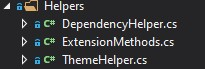
\includegraphics[scale=1.5]{Images/ARPEGOS_Helpers.jpg}
    \caption{Directorio \textit{Helpers} del proyecto \textit{ARPEGOS}}
    \label{Helpers}    
\end{figure}


\subsubsection{Resources}
En este directorio se encuentran los recursos utilizados que no dependen 
de la implementación del sistema (Figura \ref*{Resources}).

\begin{figure}[H]
    \centering
    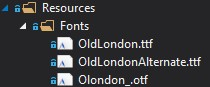
\includegraphics[scale=1.5]{Images/ARPEGOS_Resources.jpg}
    \caption{Directorio \textit{Resources} del proyecto \textit{ARPEGOS}}
    \label{Resources}    
\end{figure}\newpage

\subsubsection{Models}
La carpeta \textit{Models} contiene los modelos de la aplicación (Figura \ref*{Models}).

\begin{figure}[H]
    \centering
    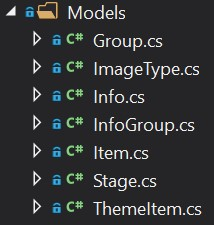
\includegraphics[scale=1]{Images/ARPEGOS_Models.jpg}
    \caption{Directorio \textit{Models} del proyecto \textit{ARPEGOS}}
    \label{Models}    
\end{figure}
\subsubsection{Themes}
Este directorio tiene las configuraciones de los distintos temas
de la aplicación (Figura \ref*{Themes}).

\begin{figure}[H]
    \centering
    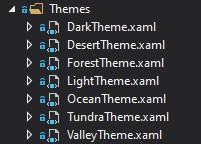
\includegraphics[scale=1.5]{Images/ARPEGOS_Themes.jpg}
    \caption{Directorio \textit{Themes} del proyecto \textit{ARPEGOS}}
    \label{Themes}    
\end{figure}
\newpage
\subsubsection{ViewModels}
En esta carpeta se encuentran los distintos modelos de vista 
de la aplicación (Figura \ref*{ViewModels}).
\begin{figure}[H]
    \centering
    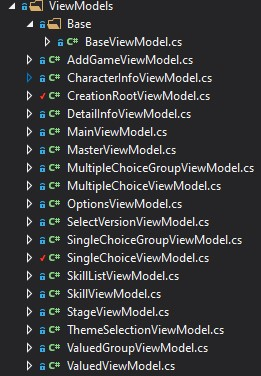
\includegraphics[scale=1]{Images/ARPEGOS_ViewModels.jpg}
    \caption{Directorio \textit{ViewModels} del proyecto \textit{ARPEGOS}}
    \label{ViewModels}    
\end{figure}

\subsubsection{Views}
Esta carpeta contiene las distintas vistas de la aplicación (Figura \ref*{Views}).

\begin{figure}[H]
    \centering
    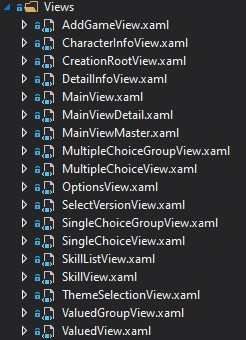
\includegraphics[scale=1]{Images/ARPEGOS_Views.jpg}
    \caption{Directorio \textit{Views} del proyecto \textit{ARPEGOS}}
    \label{Views}    
\end{figure}

\subsection{Proyecto \textit{ARPEGOS Unit Test}}
Este proyecto recoge todas las pruebas unitarias que comprueban la correcta ejecución de las funciones de la aplicación,
desglosado en la sección \ref*{UnitTest}.
\subsection{Proyecto \textit{ARPEGOS Android}}
Este proyecto contiene la estructura necesaria para implementar la aplicación en el sistema operativo \textit{Android}. Los 
elementos dispuestos aquí sólo pueden ser accedidos en caso de que la aplicación se ejecute en \textit{Android}, ya sea 
mediante un dispositivo móvil o un emulador (Figura \ref*{ARPEGOSAndroid}).

\begin{figure}[H]
    \centering
    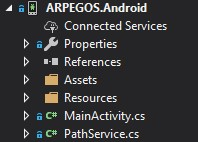
\includegraphics[scale=1.5]{Images/ARPEGOS_Android.jpg}
    \caption{Proyecto \textit{ARPEGOS Android}}
    \label{ARPEGOSAndroid}    
\end{figure}

\subsubsection{Assets}
En esta carpeta se encuentran los diferentes archivos arbitrarios, como texto, XML, fuentes, música y video en la 
aplicación (Figura \ref*{AssetsAndroid}).

\begin{figure}[H]
    \centering
    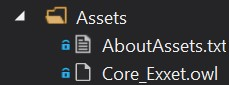
\includegraphics[scale=1.5]{Images/ARPEGOS_Android_Assets.jpg}
    \caption{Directorio \textit{Assets} del proyecto \textit{ARPEGOS Android}}
    \label{AssetsAndroid}    
\end{figure}
\newpage
\subsubsection{Resources}
Este directorio contiene los recursos \textit{predeterminados} del proyecto, que se utilzan en todos los 
dispositivos a menos que se especifique una coincidencia más específica, como el idioma por ejemplo (Figura \ref*{ResourcesAndroid}).

\begin{figure}[H]
    \centering
    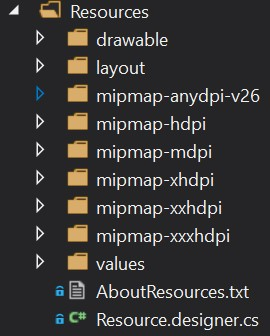
\includegraphics[scale=1]{Images/ARPEGOS_Android_Resources.jpg}
    \caption{Directorio \textit{Resources} del proyecto \textit{ARPEGOS Android}}
    \label{ResourcesAndroid}    
\end{figure}

